\chapter{Diagramele Bazei de Date OLTP}
\label{sec:diagrame_oltp}

\section{Diagrama Entitate-Relație}
\label{subsec:er_diagram}

Diagrama entitate-relație a bazei de date OLTP este prezentată mai jos:
\begin{figure}[H]
    \centering
    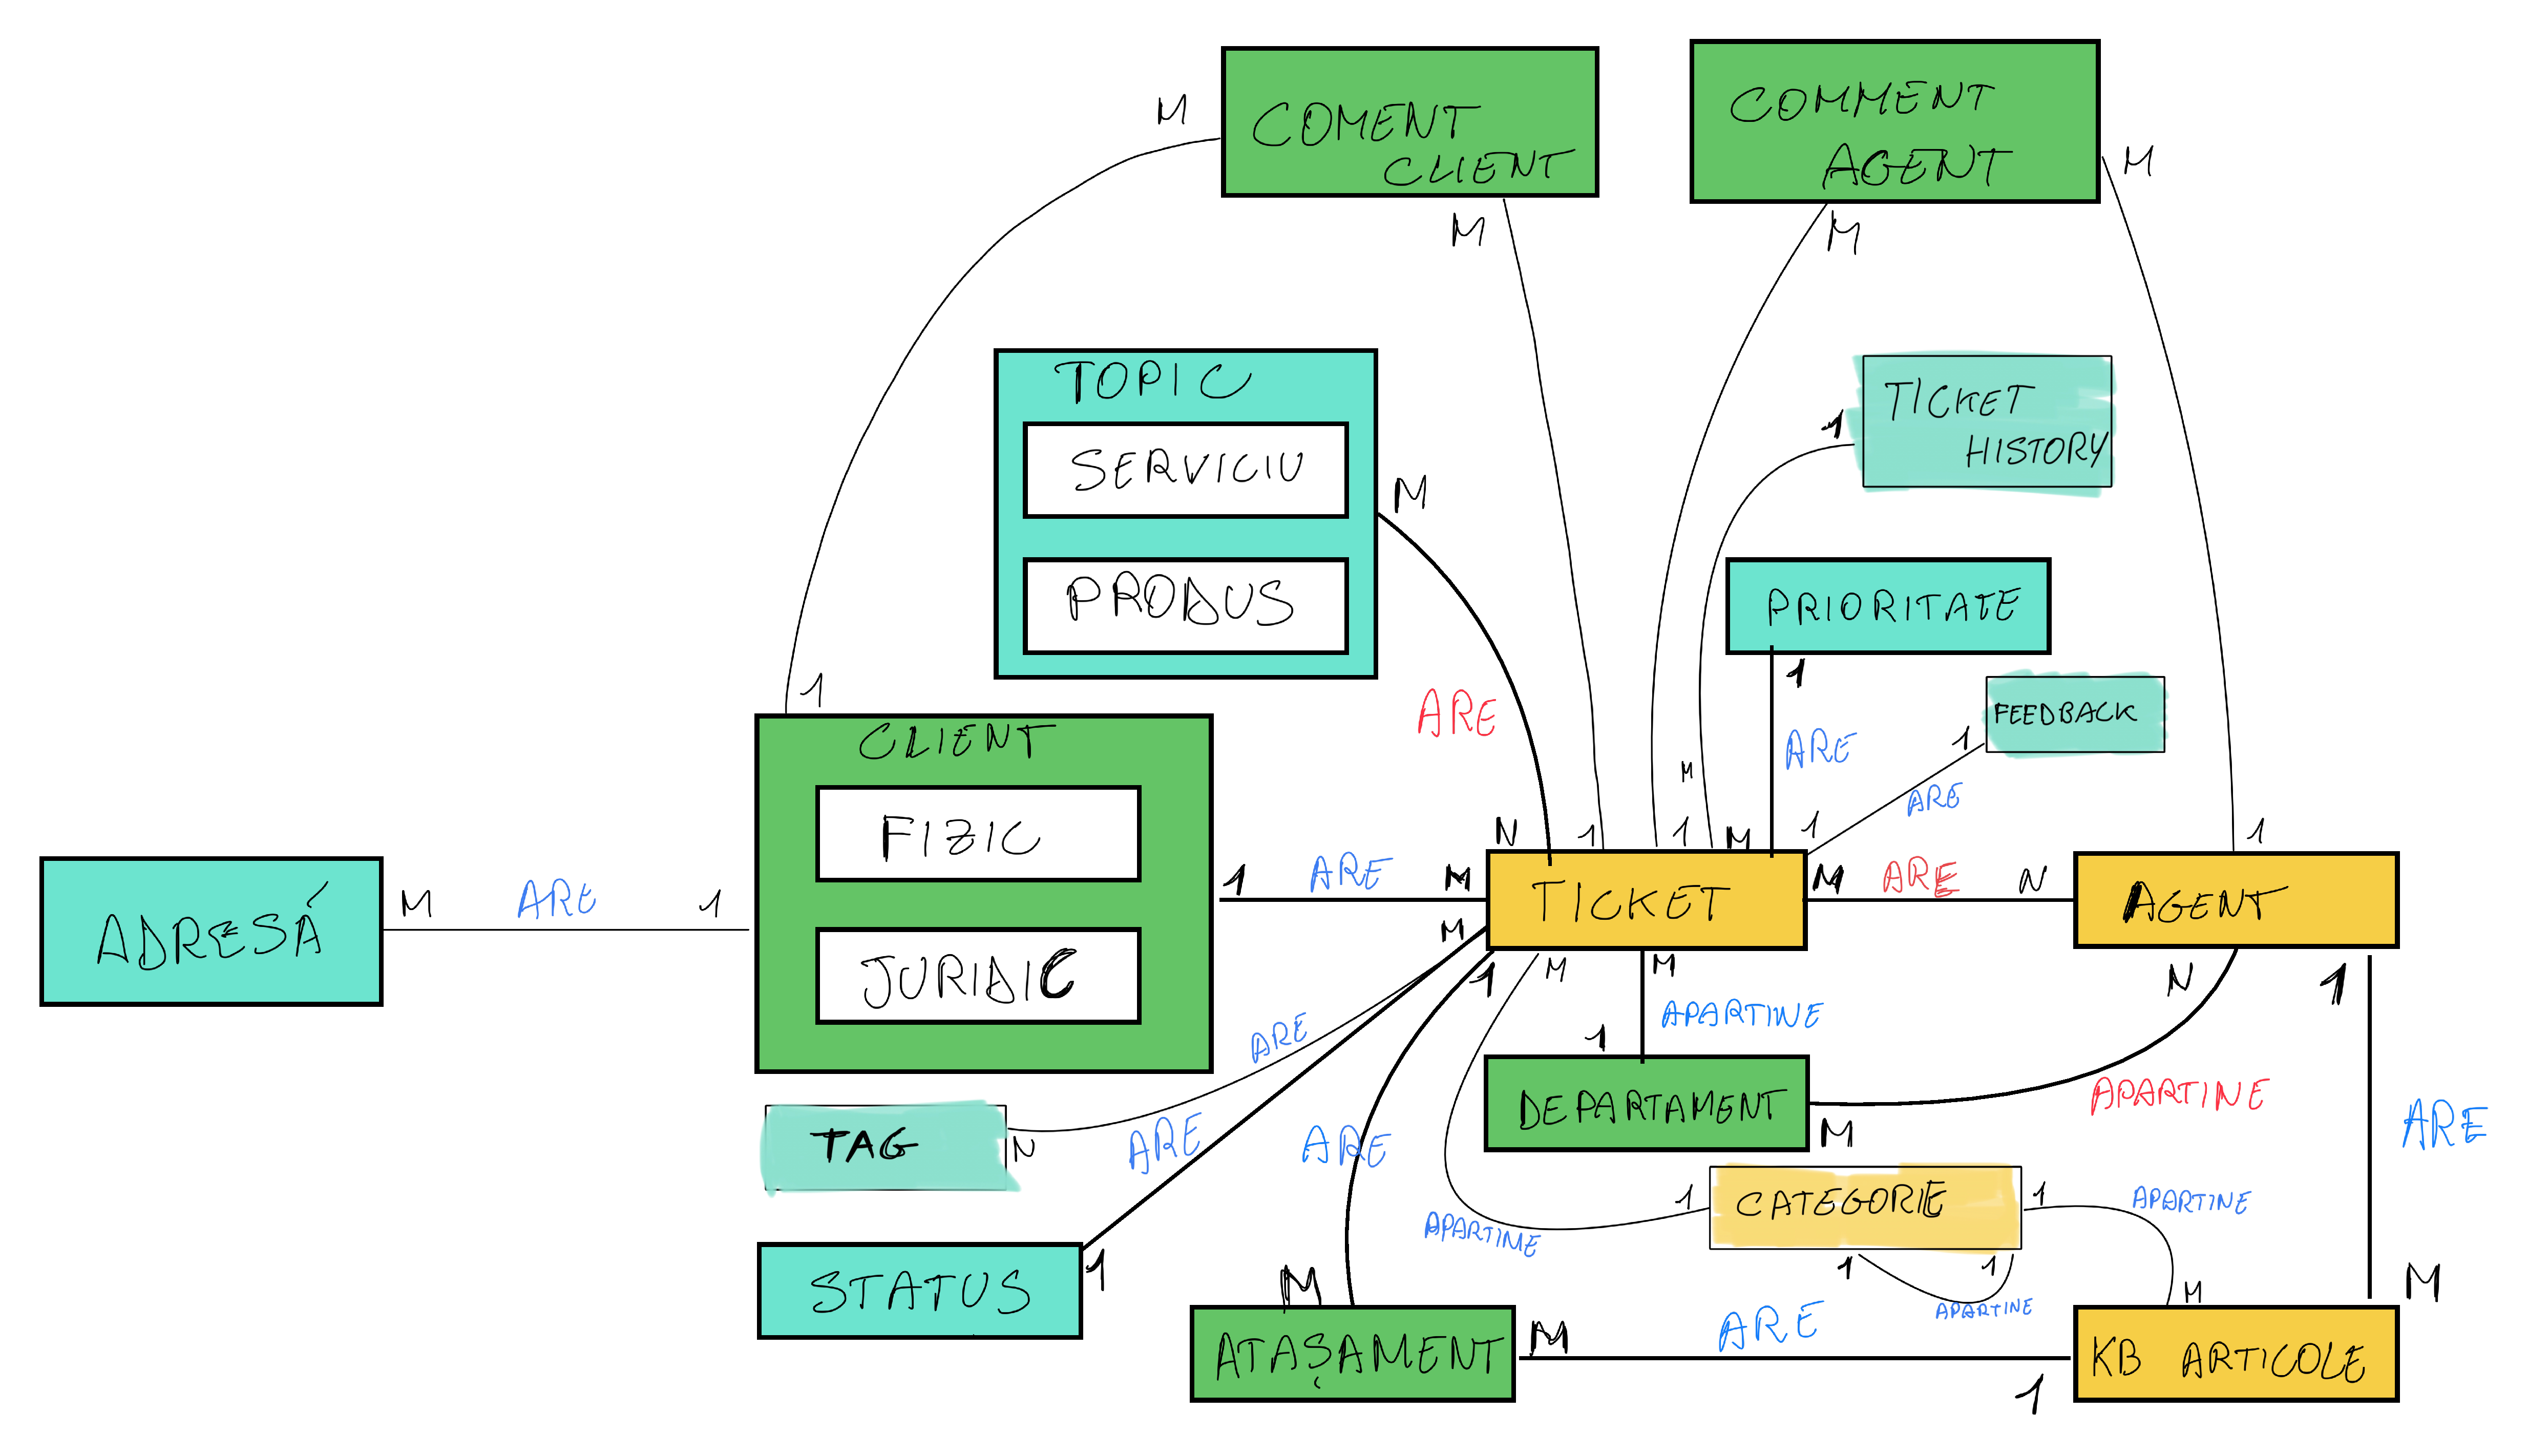
\includegraphics[width=1.0\textwidth]{../../schema/TickLy ER Diagram_Initiala.pdf}
    \caption{Diagrama Entitate-Relație a Bazei de Date OLTP}
    \label{fig:er_diagram}
\end{figure}

Această diagramă prezintă:
\begin{itemize}
    \item Toate entitățile
    \item Relațiile între entități (1:1, 1:M, M:N)
\end{itemize}

\section{Diagrama Conceptuală Extinsă}
\label{subsec:conceptual_diagram}

Diagrama conceptuală extinsă a bazei de date OLTP este prezentată mai jos:
\begin{figure}[H]
    \centering
    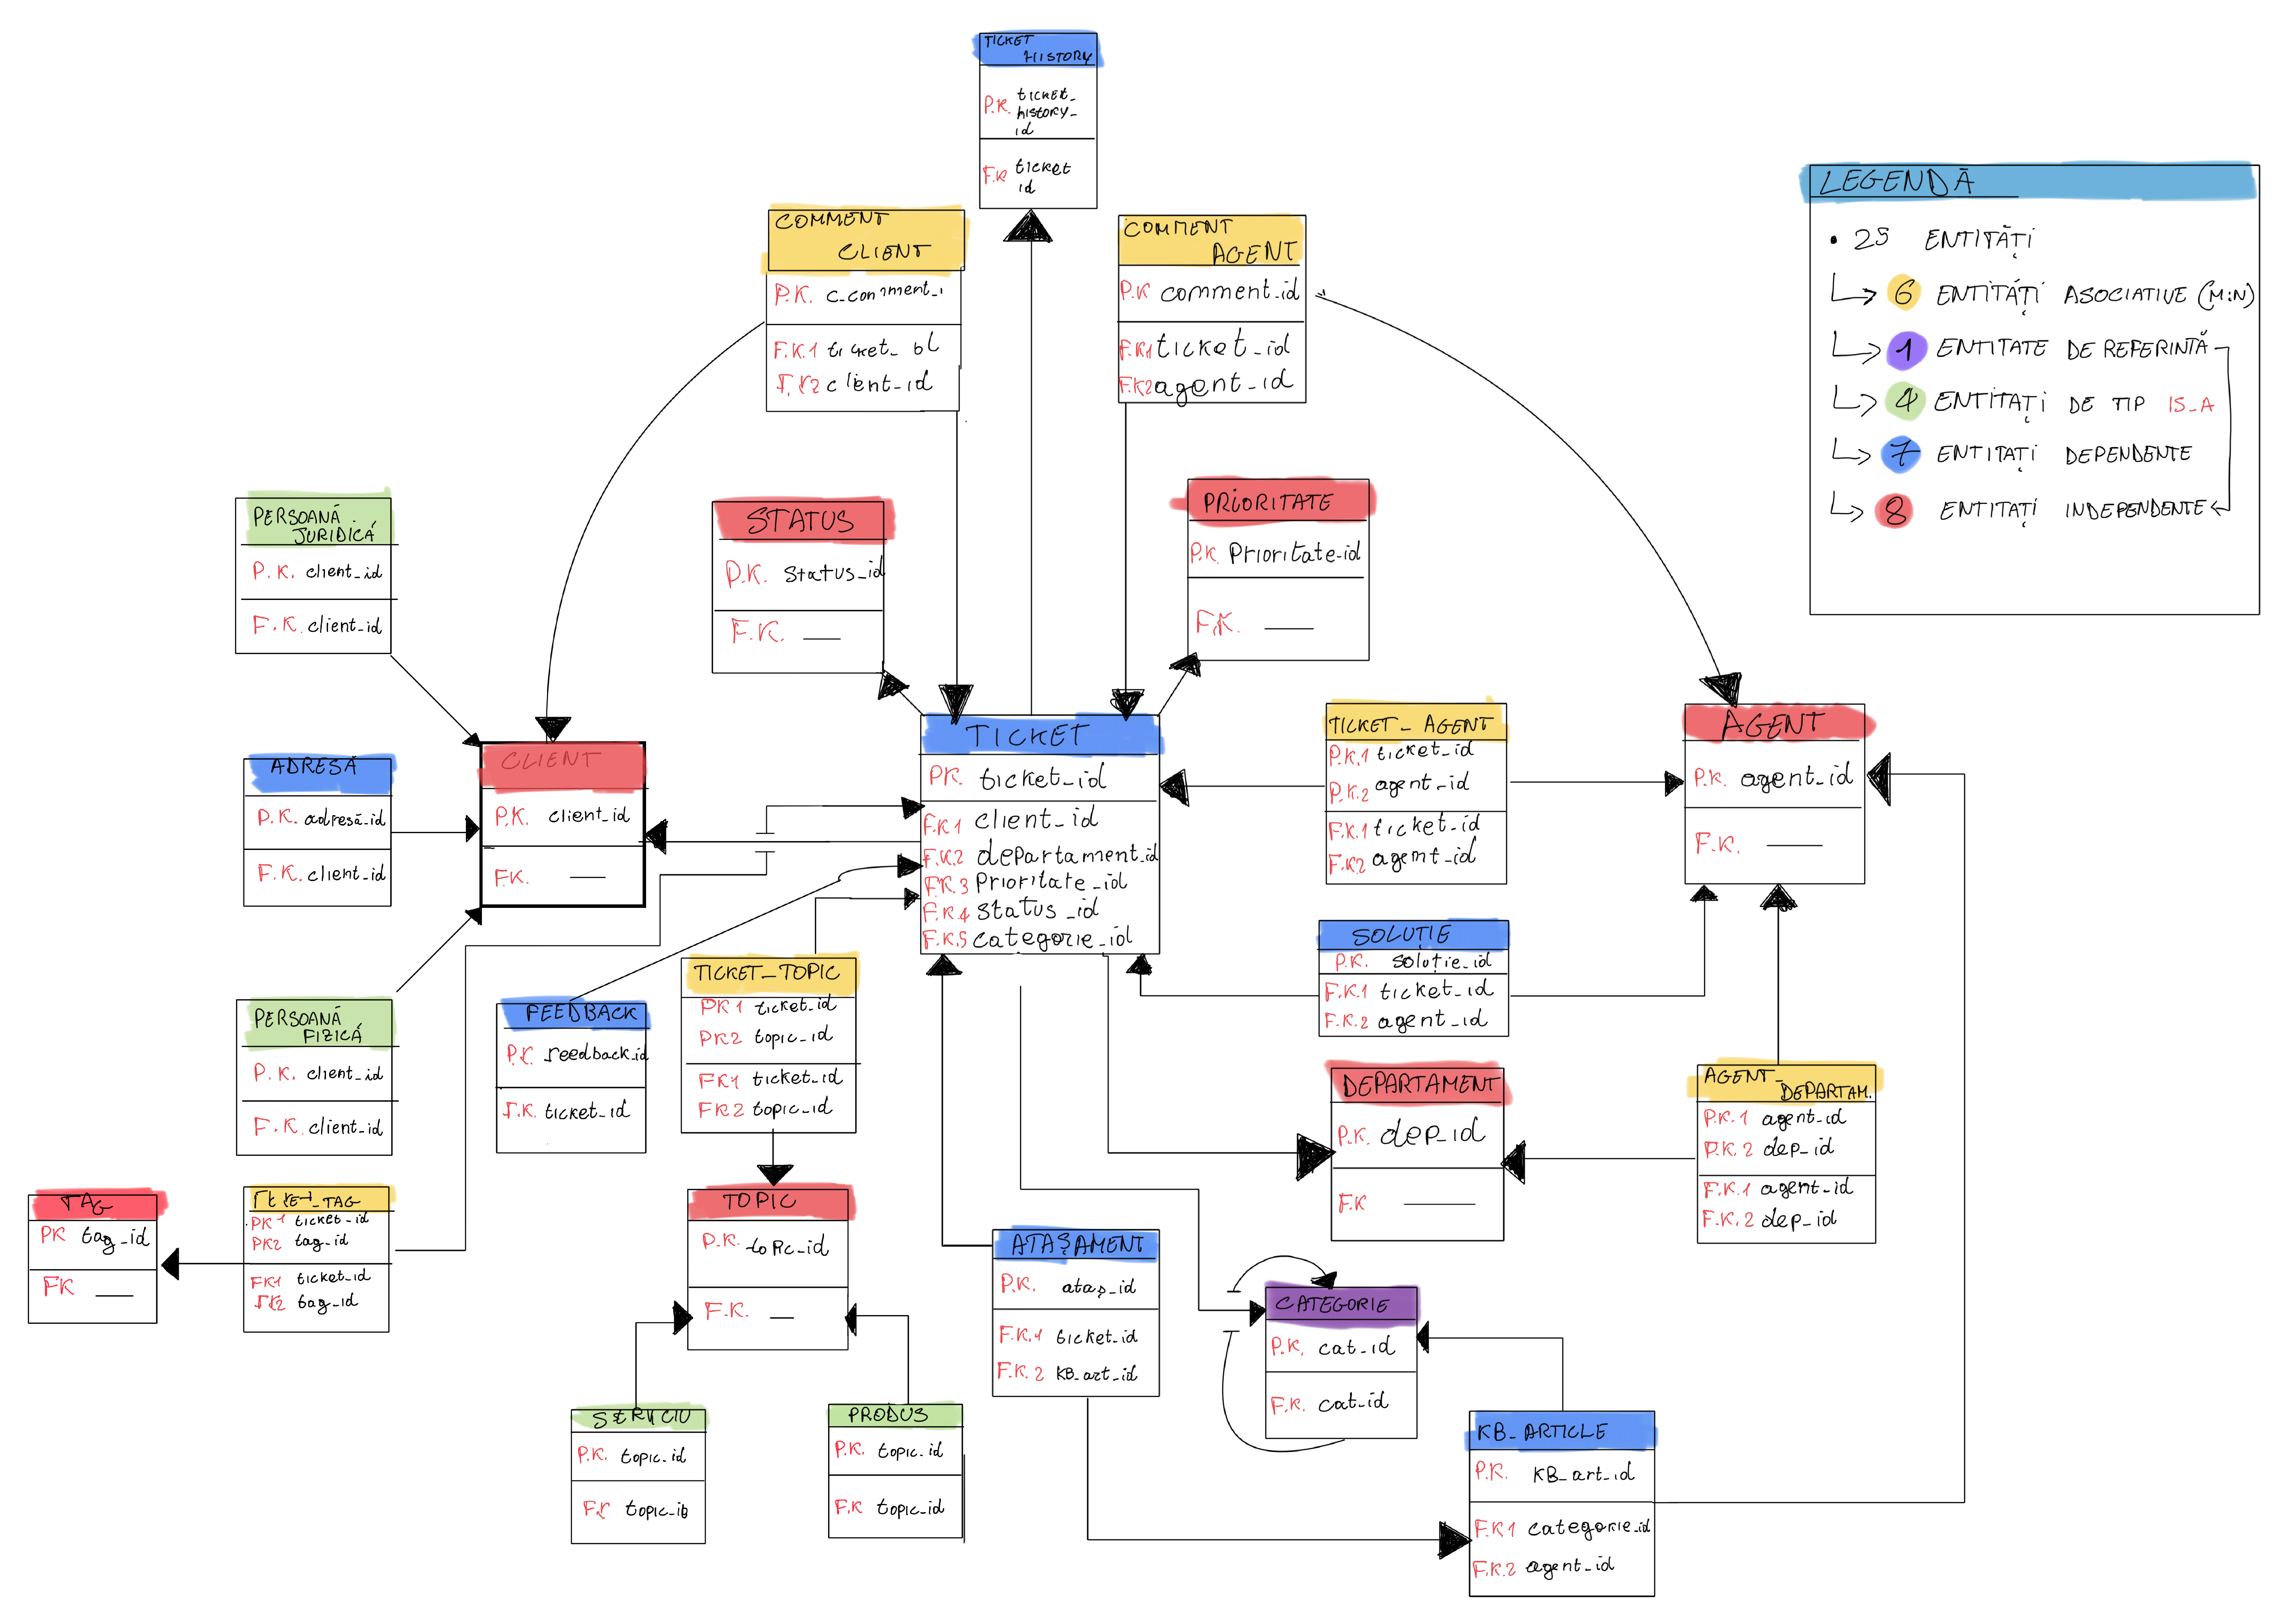
\includegraphics[width=1.0\textwidth]{../../schema/TickLy Conceptuală Extinsă.pdf}
    \caption{Diagrama Conceptuală Extinsă a Bazei de Date OLTP}
    \label{fig:conceptual_diagram}
\end{figure}

Baza de date OLTP conține următoarele: 

\subsubsection{Entități independente}

\begin{enumerate}
    \item \textbf{CLIENT} — entitate părinte pentru clienți
    \item \textbf{AGENT} — agenții de suport
    \item \textbf{PRIORITATE} — nivelurile de prioritate ale tichetelor
    \item \textbf{STATUS} — statusurile tichetelor
    \item \textbf{TOPIC} — entitate părinte pentru topic-urile asociate tichetelor
    \item \textbf{CATEGORIE} — categoriile pentru organizarea tichetelor
    \item \textbf{TAG} — tag-uri pentru etichetarea tichetelor
    \item \textbf{DEPARTAMENT} — departamentele organizației
\end{enumerate}

\textbf{Nota:} Categorie este o entitate de referinta catre categoria parinte.

\subsubsection{Entități dependente}

\begin{enumerate}
    \item \textbf{TICKET} — tichetele de suport
    \item \textbf{TICKET\_HISTORY} — istoricul evenimentelor pe tichete (audit trail)
    \item \textbf{ATASAMENT} — atașamentele la tichete sau la articole KB
    \item \textbf{KB\_ARTICLE} — articole din baza de cunoștințe (documentație)
    \item \textbf{FEEDBACK} — feedback-urile clienților la tichete (rating, comentariu)
    \item \textbf{SOLUTIE} — soluțiile înregistrate la tichete rezolvate
    \item \textbf{ADRESA} — adresele clienților (facturare, livrare, sediu)
\end{enumerate}

\subsubsection{Entități de tip IS-A}

\begin{enumerate}
    \item \textbf{CLIENT $\rightarrow$ CLIENT\_FIZICA / CLIENT\_JURIDICA} — clienți persoane fizice sau juridice
    \item \textbf{TOPIC $\rightarrow$ TOPIC\_SERVICIU / TOPIC\_PRODUS} — topic-uri de tip serviciu sau produs
\end{enumerate}

\subsubsection{Relații Many-to-Many}

Sistemul conține următoarele relații many-to-many (M:N), implementate prin tabele asociative:

\begin{itemize}
    \item \textbf{Ticket $\leftrightarrow$ Agent} (prin \texttt{TICKET\_AGENT}) - un ticket poate fi asignat mai multor agenți, iar un agent poate lucra la mai multe tichete
    \item \textbf{Ticket $\leftrightarrow$ Topic} (prin \texttt{TICKET\_TOPIC}) - un ticket poate fi asociat cu mai multe topic-uri, iar un topic poate fi asociat cu mai multe tichete
    \item \textbf{Agent $\leftrightarrow$ Departament} (prin \texttt{AGENT\_DEPARTAMENT}) - un agent poate aparține mai multor departamente, iar un departament poate avea mai mulți agenți
    \item \textbf{Ticket $\leftrightarrow$ Tag} (prin \texttt{TICKET\_TAG}) - un ticket poate avea mai multe tag-uri, iar un tag poate fi asociat cu mai multe tichete
    \item \textbf{Comment $\leftrightarrow$ Client} (prin \texttt{COMMENT\_CLIENT}) - un ticket poate avea mai multe comentarii de la client, iar un client poate avea mai multe comentarii la tichete
    \item \textbf{Comment $\leftrightarrow$ Agent} (prin \texttt{COMMENT\_AGENT}) - un ticket poate avea mai multe comentarii de la agent, iar un agent poate avea mai multe comentarii la tichete
\end{itemize}
